\chapter{Theoretical background}
\label{chap:theoretical_background}
\section{Serialisation and Deserialisation}
\label{tb:serialisation_deserialisation}
Before discussing the specific techniques used in the FlatCityBuf format, it is important to understand the general principles of serialisation and deserialisation.

The terminology for data conversion processes varies across different programming ecosystems. Terms such as serialisation, pickling, marshalling, and flattening are often used interchangeably, though with subtle differences depending on the context. \citet{cpp_serialization} describes it from an object-oriented perspective as converting objects to a storable or transmittable format and later reconstructing them. \citet{py_serialization} refers to this process as "pickling" in the Python ecosystem. For clarity in this thesis, we adopt the definition provided by \citet{viotti_2022}:

\begin{quote}
  "Serialization is the process of translating a data structure into a bit-string (a sequence of bits) for storage or transmission purposes."
\end{quote}

Deserialisation is the reverse process of serialisation, where the bit-string is converted back into the original data structure.

\section{Zero-copy}
\label{tb:zero_copy}
Zero-copy is a technique used to avoid copying data from one memory location to another. While, the term "Zoro-copy" is used in many contexts of computer science, \citet{song2012performance}  and \citet{brose_2008_zerocopy} provide a more detailed explanation of the concept.

\subsection{Typical Data Transfer with read/write}
In conventional I/O operations, data typically traverses multiple memory regions, each requiring a separate copy operation:

\begin{itemize}
  \item Data is copied from storage devices into kernel buffer cache
  \item From kernel buffer, data is copied to user-space application buffers
  \item For network transmission, data may be copied again to network buffers
\end{itemize}

This multi-stage copying introduces significant overhead, particularly for large datasets or high-throughput applications. Each copy operation consumes CPU cycles, memory bandwidth, and increases latency \citep{song2012performance}. For applications working with large 3D city models, this overhead can substantially degrade performance.

\subsection{Zero-copy Techniques}
\label{tb:zero_copy_techniques}
\todo{Check if this is correct, atm I briefly glanced over the literature added bullect points}
Zero-copy approaches optimize this data path by eliminating unnecessary copy operations. While "zero-copy" as a term suggests complete elimination of copying, in practice, different techniques achieve varying degrees of copy reduction:

\begin{itemize}
  \item \textbf{Memory-mapped \ac{io}}: Maps files directly into process address space, allowing direct access without explicit read/write operations
  \item \textbf{Direct \ac{io}}: Bypasses the kernel buffer cache for specific workloads
  \item \textbf{Scatter-gather \ac{io}}: Reads data directly into discontiguous memory regions
  \item \textbf{Shared memory}: Provides common address space for inter-process communication
  \item \textbf{In-place parsing}: Processes data structures without creating intermediate copies
\end{itemize}

Modern serialization formats like FlatBuffers implement zero-copy through carefully designed memory layouts that allow direct access to serialized data without requiring a separate deserialization step. This approach is particularly valuable for geospatial applications that routinely handle large datasets.
\section{Endianness}
\label{tb:endianness}
Endianness (or "byte-order") refers to the order in which bytes are stored in memory when representing multi-byte values. The terminology was introduced by \citet{danny_cohen_1981}.

In computing, endianness becomes significant when multi-byte data types (such as 16-bit integers or 32-bit floats) must be stored in memory or transmitted across networks. There are two primary byte ordering systems:

\begin{itemize}
  \item \textbf{Little-endian}: Stores the least significant byte at the lowest memory address, followed by increasingly significant bytes. This is the ordering used by Intel processors that dominate desktop and server computing. For example, the 32-bit integer \texttt{0x12345678} would be stored in memory as \texttt{0x78}, \texttt{0x56}, \texttt{0x34}, \texttt{0x12}.

  \item \textbf{Big-endian}: Stores the most significant byte at the lowest memory address. This approach is often called ``network byte order'' because Internet protocols typically require data to be transmitted in big-endian format. For example, the same 32-bit integer \texttt{0x12345678} would be stored as \texttt{0x12}, \texttt{0x34}, \texttt{0x56}, \texttt{0x78}.
\end{itemize}

A useful analogy is date notation: little-endian resembles the European date format (31 December 2050), while big-endian resembles the ISO format (2050-12-31), with the most significant part (year) first \citep{endianness_mdn}.

\section{Indexing algorithms}
\label{tb:indexing_algorithms}

\subsection{Indexing Strategy Evaluation}

Several indexing strategies were evaluated to determine the most appropriate approach for the FlatCityBuf format:

\begin{table}[ht]
  \centering
  \caption{Comparison of Indexing Strategies}
  \begin{tabular}{l|c|c|c|c}
    \hline
    \textbf{Strategy} & \textbf{Exact Match} & \textbf{Range Query} & \textbf{Space Efficiency} & \textbf{HTTP Suitability} \\
    \hline
    Hash Tables & $O(1)$ & Poor & Medium & Poor \\
    Sorted Array & $O(\log n)$ & Good & Excellent & Limited \\
    Binary Search Tree & $O(\log n)$ & Good & Good & Limited \\
    B-tree/B+tree & $O(\log_B n)$ & Excellent & Good & Excellent \\
    \hline
  \end{tabular}
  \label{tab:indexing_strategies}
\end{table}

Initial implementation used a sorted array with binary search for its simplicity and space efficiency. However, performance testing revealed significant I/O latency issues when accessing this structure over HTTP, as each binary search step potentially required a separate HTTP request. This insight led to a re-evaluation of the indexing approach.

\section{Binary Search}
\label{tb:binary_search}

Binary search is a fundamental algorithm for finding elements in a sorted array. The classic implementation follows a simple approach: compare the search key with the middle element of the array, then recursively search the left or right half depending on the comparison result \citep{binary_search}.
\begin{algorithm}
  \KwIn{A sorted array, a target value, left and right bounds}
  \KwOut{The index where the target value should be inserted}
  \BlankLine
  \While{left $<$ right}
  {
    mid $\leftarrow$ (left + right) / 2\;
    \If{array[mid] $\geq$ target}
    {
      right $\leftarrow$ mid\;
    }
    \Else
    {
      left $\leftarrow$ mid + 1\;
    }
  }
  \Return{left}
  \caption{Classic Binary Search}%
  \label{alg:binary_search}
\end{algorithm}

The time complexity of binary search is logarithmic—the height of the implicit binary search tree is $\log_2(n)$ for an array of size $n$. While this is theoretically efficient, the actual performance suffers when implemented on modern hardware due to memory access patterns. Each comparison requires the processor to fetch a new element, potentially causing a cache miss. In the worst case, the number of memory read operations will be proportional to the height of the tree, with each read potentially requiring access to a different cache line or disk block \citep{binary_search}.

This inefficiency is particularly problematic when binary search is implemented on external memory or over HTTP, where each access incurs significant latency. The sorted array representation with binary search does not take advantage of CPU cache locality, as consecutive comparisons frequently access distant memory locations.

\subsection{Eytzinger Layout}
\label{tb:eytzinger_layout}

While preserving the same algorithmic idea as binary search, the Eytzinger layout (also known as a complete binary tree layout or level-order layout) rearranges the array elements to match the access pattern of a binary search \citep{binary_search}. Instead of storing elements in sorted order, it places them in the order they would be visited during a level-order traversal of a complete binary tree.

This layout significantly improves memory access patterns. When the array is accessed in the sequence of a binary search operation, adjacent accesses often refer to elements that are in the same or adjacent cache lines. This spatial locality enables effective hardware prefetching, allowing the CPU to anticipate and load required data before it is explicitly accessed, thus reducing latency \citep{binary_search}.

The \autoref{fig:eytzinger_layout} shows how the layout looks when applied to binary search. The \autoref{fig:eytzinger_layout2} shows that the algorithm starts from the first element and then jumps to either $2k$ or $2k+1$ depending on the comparison result.

\begin{figure}[ht]
  \centering
  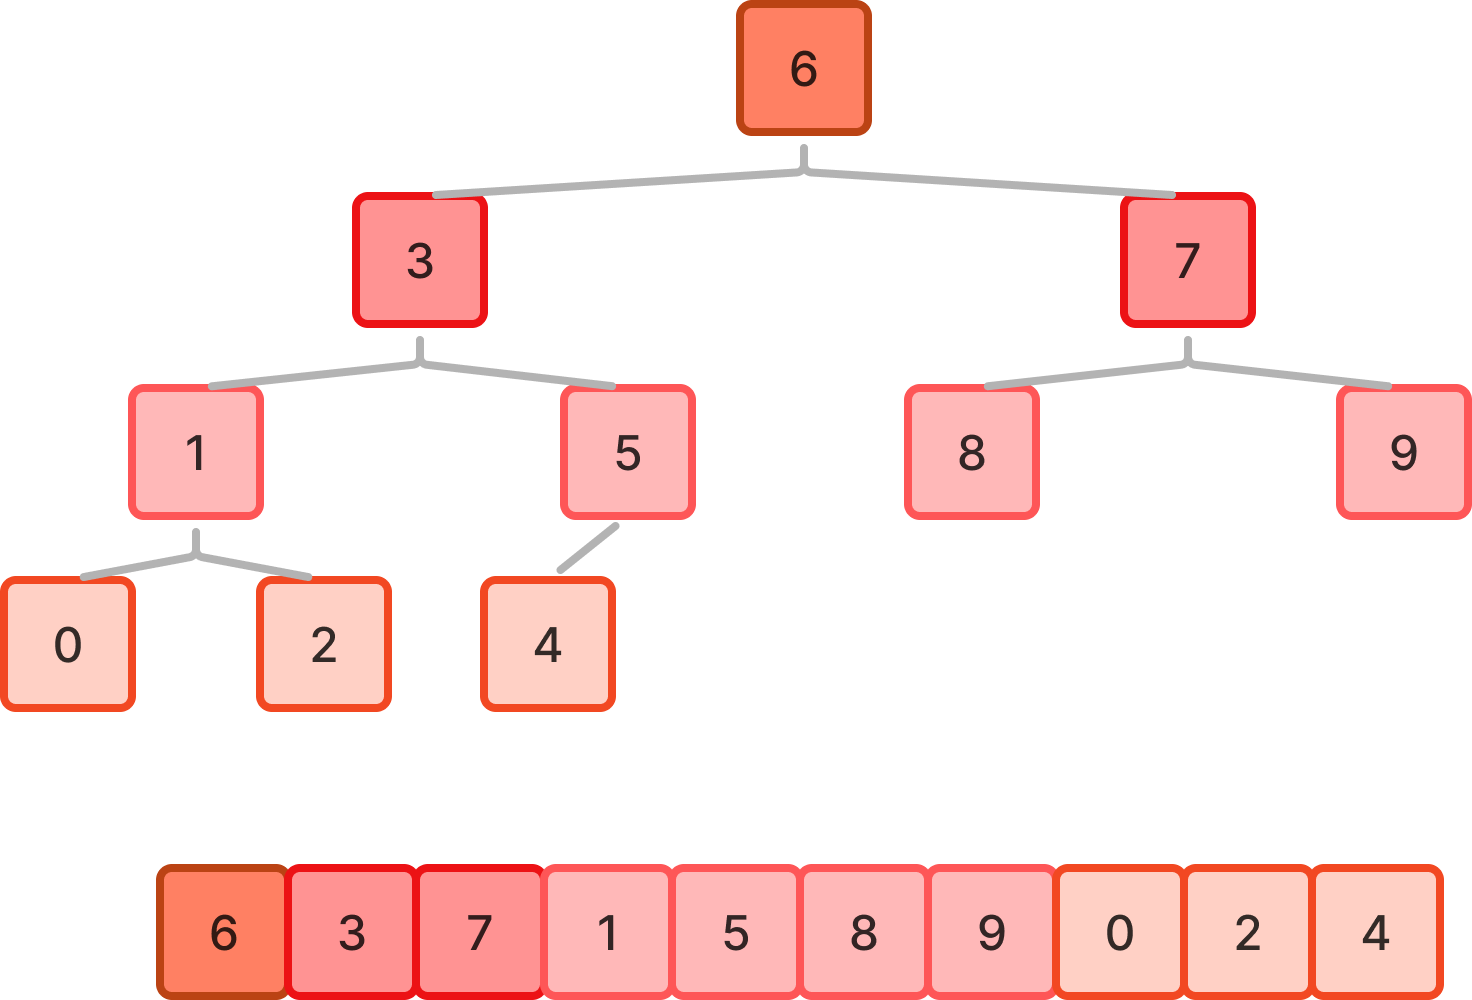
\includegraphics[width=0.5\textwidth]{figs/related_work_theoretical_bg/eytzinger_layout.png}
  \caption{Eytzinger layout as conceptual representation as tree and actual data layout (derived from \citet{binary_search})}
  \label{fig:eytzinger_layout}
\end{figure}
\begin{figure}[ht]
  \centering
  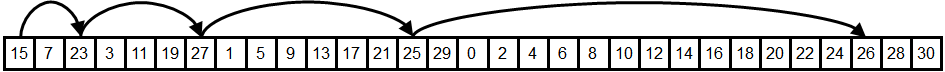
\includegraphics[width=0.5\textwidth]{figs/related_work_theoretical_bg/eytzinger_layout2.png}
  \caption{Binary search traversal pattern in Eytzinger layout (derived from \citet{binary_search})}
  \label{fig:eytzinger_layout2}
\end{figure}

\section{\texorpdfstring{\ac{s+tree}}{S+tree}}
\label{tb:static_btree}

\subsection{B-Tree/B+Tree Layout}
\label{tb:btree_layout}

While the Eytzinger layout improves cache utilization for binary search, the number of memory read operations remains proportional to the height of the tree—$\log_2(n)$ for $n$ elements. This is still suboptimal for large datasets, especially when the access pattern involves disk \ac{io} or remote data access \citep{static_b_trees}.

B-Trees and their variants address this limitation by storing multiple keys in each node, effectively reducing the height of the tree. In a B-Tree of order $k$ (where each node can contain up to $k-1$ keys), the height of the tree is reduced from $\log_2(n)$ to $\log_k(n)$. This represents a reduction factor of $\log_k/\log_2 = \log_2(k)$ times compared to a binary search tree.

The key insight is that fetching a single node still takes roughly the same time regardless of whether it contains one key or multiple keys, as long as the entire node fits into a single memory block or disk page. By packing multiple keys into each node, B-Trees significantly reduce the number of disk or memory accesses required to locate an element.

B+Trees are a variant of B-Trees specifically optimized for range queries and sequential access patterns. In a B+Tree:
\begin{itemize}
  \item Internal nodes contain up to $B$ keys that serve as routing information, with each key associated with one of the $(B+1)$ pointers to child nodes. Each key at position $i$ represents the smallest key in the subtree pointed to by the $(i+1)$-th child pointer.
  \item Leaf nodes store the actual data with up to $B$ key-value pairs and include a pointer to the next leaf node, enabling efficient sequential traversal for range queries.
\end{itemize}

This linked structure of leaf nodes enables B+Trees to efficiently support range queries by traversing from one leaf to the next without needing to return to higher levels of the tree.

\subsection{\texorpdfstring{\ac{s+tree}}{S+tree}}
\label{tb:stree}

The \ac{s+tree} approach, introduced by Algorithmica \citep{static_b_trees}, builds upon the B+Tree concept but is specifically designed for static datasets where the tree structure never changes after construction. Unlike traditional B+Trees that use explicit pointers between nodes, the Static B+Tree uses an implicit structure where child positions are calculated mathematically.

This is possible because:
\begin{itemize}
  \item The tree is constructed once and never modified (static)
  \item The number of elements is known in advance
  \item The tree can be maximally filled with no empty slots
  \item Child positions follow a predictable pattern based on the block size
\end{itemize}

For a \ac{s+tree} with block size $B$, a node with index $k$ has its children at indices calculated by a simple formula: $\text{child}_i(k) = k \cdot (B+1) + i + 1$ for $i \in [0, B]$ \citep{static_b_trees}. This eliminates the need to store and fetch explicit pointer values, further reducing memory usage and improving cache efficiency.

The S+Tree layout aligns with modern hardware characteristics where:
\begin{itemize}
  \item The latency of fetching a single byte is comparable to fetching an entire cache line (64 bytes)
  \item Disk and network I/O operations have high initial latency but relatively low marginal cost for additional bytes
  \item CPU cache lines typically hold multiple array elements (e.g., 16 integers in a 64-byte cache line)
\end{itemize}

By loading a block of $B$ elements at once and performing a local search within that block, S+Trees reduce the total number of cache misses or disk accesses to $\log_B(n)$ instead of $\log_2(n)$—a significant reduction for large datasets.

The S+Tree layout achieves up to 15× performance improvement over standard binary search implementations while requiring only 6-7\% additional memory \citep{static_b_trees}. This makes it particularly valuable for applications that perform frequent searches on large, relatively static datasets, especially when accessed over high-latency connections. For more detailed implementation strategies of S+Tree, \citet{koerkamp_2024} provides comprehensive explanations and practical considerations.